% Part: sets-functions-relations
% Chapter: arithmetization
% Section:reals

\documentclass[../../../include/open-logic-section]{subfiles}

\begin{document}

\olfileid{sfr}{arith}{real}
\olsection{De reële getallenlijn}
De volgende stap is de constructie van de reële getallen uit de
rationale getallen. Eerst moeten we begrijpen wat de reële getallen
\emph{kenmerkt}.
De reële getallen gedragen zich in veel opzichten hetzelfde als de
rationale getallen. (Technisch zijn beide voorbeelden van \emph{geordende
lichamen}; zie \olref[check]{orderedfield} voor de definitie.) Wie de
opgaven bij \olref[sfr][siz][]{chap} heeft gemaakt, weet dat er strikt
meer reële dan rationale getallen zijn, dus dat
$\cardless{\Rat}{\Real}$. Cantor bewees dit als eerste. Al ongeveer
tweeënhalf millennium is echter bekend dat er irrationale getallen
bestaan, dat wil zeggen reële getallen die niet rationaal zijn. Er
geldt namelijk:
%\footnote{Now: ``$\sqrt{2}$'' equally refers to both the positive and the negative roots; but in the next few pages, I'll forget about this, and consider only the positive root.}
\begin{thm}\ollabel{root2irrational}
$\sqrt{2}$ is niet rationaal, dat wil zeggen $\sqrt{2} \notin \Rat$.
\end{thm}
\begin{proof}
Stel, om een tegenspraak af te leiden, dat $\sqrt{2}$ rationaal is.
Dan is $\sqrt{2} = \nicefrac{m}{n}$ voor zekere natuurlijke getallen
$m$ en $n$. We kunnen $m$ en $n$ zo klein mogelijk kiezen; de breuk
kan dan niet verder worden vereenvoudigd. Omwerken geeft $m^{2} =
2n^{2}$. Vanaf hier
kunnen we het bewijs op twee manieren voltooien:
\emph{Ten eerste meetkundig} (naar Tennenbaum).\footnote{Dit bewijs
wordt vermeld door \cite{Conway2006}.} Beschouw de volgende vierkanten:
\begin{center}	
	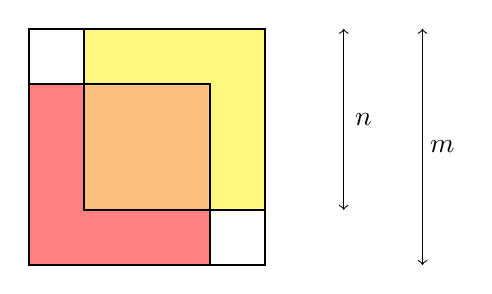
\begin{tikzpicture}
		\draw[thick] (0,0) rectangle (3,3);
		\draw[thick, fill=red!50] (0,0) rectangle (2.3,2.3);
		\draw[thick, fill=yellow!50] (0.7,0.7) rectangle (3, 3);
		\draw[thick, fill=orange!50] (0.7,0.7) rectangle (2.3, 2.3);
		\draw[<->] (4, 0.7)--(4, 3);
		\node at (4.25, 1.85) (n) {$n$};
		\draw[<->] (5, 0)--(5, 3);
		\node at (5.25, 1.5) (m) {$m$};
	\end{tikzpicture}
\end{center}
Omdat $m^2 = 2n^2$, heeft het gebied waarin de twee vierkanten met
zijde $n$ overlappen dezelfde oppervlakte als het gebied dat door
geen van beide vierkanten wordt bedekt. De oppervlakte van het oranje
vierkant is dus gelijk aan de som van de oppervlakten van de twee
niet-ingekleurde vierkanten. Als het oranje vierkant zijde $p$ heeft
en elk niet-ingekleurd vierkant zijde $q$, dan is $p^2 = 2q^2$. Nu is
echter $\sqrt{2} = \nicefrac{p}{q}$, waarbij $p < m$, $q < n$ en $p, q
\in \Nat$. Dit is in tegenspraak met de keuze van $m$ en $n$ als zo
klein mogelijk.
\emph{Ten tweede formeel.} Uit $m^{2} = 2n^{2}$ volgt dat $m$ even is.
(Als $x$ oneven is, is eenvoudig aan te tonen dat $x^2$ oneven is.)
Er geldt dus $m = 2r$ voor een zekere $r \in \Nat$. Omwerken geeft
$2r^2 = n^2$,
		%				\begin{align*}
		%					(2q)^{2} &= 2n^{2}\\
		%					4q^{2} &= 2n^{2}\\
		%					2q^{2} &= n^{2}
		%				\end{align*}
zodat ook $n$ even is. Zowel $m$ als $n$ is dus even, en daarom kan de
breuk $\nicefrac{m}{n}$ \emph{wel} verder worden vereenvoudigd. Dit
is een tegenspraak.
\end{proof}
Dit bewijs met een diagram voert ons ook terug naar
\olref[his][set][mythology]{sec}. Tennenbaum (1927--2006) was een door
en door moderne wiskundige. Toch is het bewijs onmiskenbaar fraai en
volledig sluitend, en doet het een beroep op meetkundige intuïtie.
Hoe dan ook zijn de reële getallen ``omvangrijker'' dan de rationale
getallen. In zekere zin vertonen de rationale getallen ``gaten'', die
door de reële getallen worden opgevuld. Weierstrass zag in dat dit één
eigenschap van de reële getallen beschrijft die ze van de rationale
getallen onderscheidt, namelijk de volledigheidseigenschap:
\emph{Iedere niet-lege verzameling reële getallen met een bovengrens
heeft een kleinste bovengrens.}
Het is eenvoudig in te zien dat de rationale getallen de
volledigheidseigenschap niet hebben. Beschouw bijvoorbeeld de
verzameling rationale getallen kleiner dan $\sqrt{2}$:
\[
	\Setabs{p \in \Rat}{p^2 < 2 \text{ of }p < 0}
\]
Deze verzameling heeft een rationale bovengrens; al haar !!{element}en
zijn bijvoorbeeld kleiner dan $3$. Maar wat is haar kleinste
bovengrens? We zouden `$\sqrt{2}$' willen antwoorden, maar we hebben
zojuist gezien dat $\sqrt{2}$ \emph{niet} rationaal is. Er bestaat ook
geen \emph{kleinste} rationaal getal groter dan $\sqrt{2}$. De
verzameling heeft dus wel een bovengrens, maar geen kleinste
bovengrens. De rationale getallen missen bijgevolg de
volledigheidseigenschap.
Het continuüm zou daarentegen, intuïtief bezien, de
volledigheidseigenschap moeten hebben. We willen niet alleen dat
$\sqrt{2}$ een reëel getal is, maar ook dat alle ``gaten'' in de
rationale getallenlijn worden opgevuld. Het continuüm zelf moet dus
geen ``gaten'' bevatten. Dat is precies wat volledigheid ons zal geven.
\end{document}